% =====================================================================
%  main.tex — WRAPPER (wiring). NIE pisz tu treści.
%  Treść jest w tresc/*.tex; wygląd w formatka/slayer.sty (bez zmian, slay-paper c2497c79).
%  Wersja angielska: babel dostaje dodatkowo english, a dokument przełącza język.
% =====================================================================
\documentclass[11pt,a4paper]{article}

\PassOptionsToPackage{english}{babel}
\usepackage{formatka/slayer}   % <-- FORMATKA (jedyne miejsce sterujące wyglądem)
\hypersetup{pdftitle={Slayer 150 1.01: Choosing a Training Recipe with Decision Rules Fixed Before Each Result}, pdfauthor={Arkadiusz Słota}, pdfcreator={SlayerLabs}, pdfproducer={SlayerLabs}}
\pdfinfoomitdate=1
\pdftrailerid{}
\pdfsuppressptexinfo=-1

\begin{document}
\selectlanguage{english}

% =====================================================================
%  Title page — title, author, hero chart with caption.
% =====================================================================
\begin{titlepage}
\centering
\vspace*{1.0cm}

\slayertitle
  {Slayer 150 1.01:\\ choosing a training recipe with decision rules\\ fixed before each result}%
  {Arkadiusz Słota, Fabryka AI}%
  {Draft, 7 October 2026 --- training in progress}

\vspace{0.8cm}

\begin{figure}[h]
  \centering
  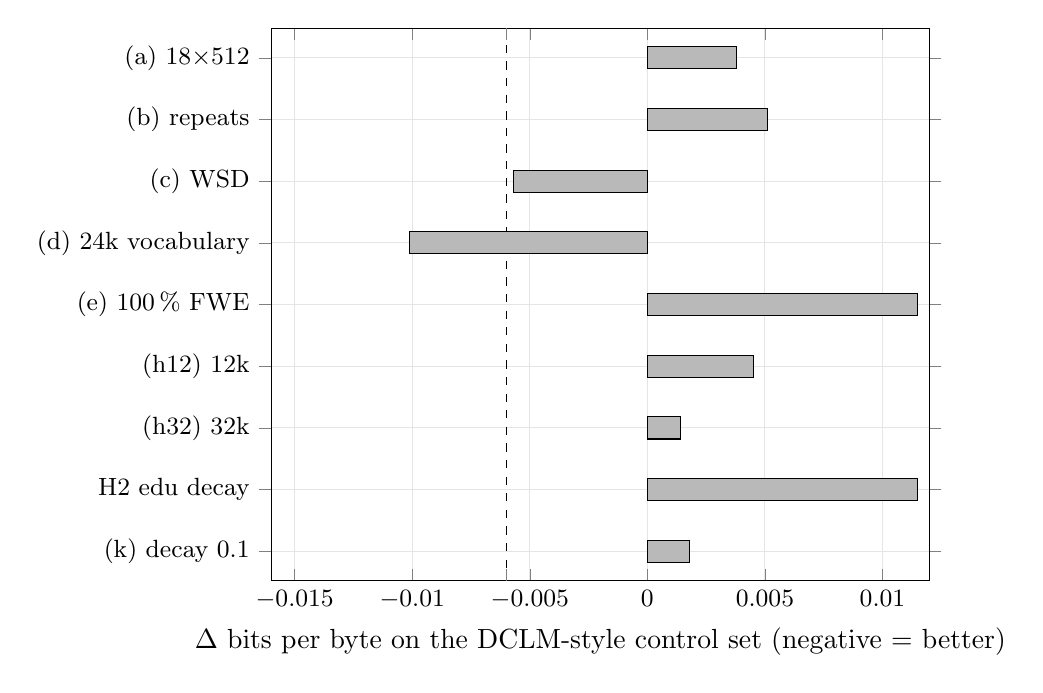
\begin{tikzpicture}
    \begin{axis}[
        xbar, width=0.82\linewidth, height=8.6cm,
        xlabel={$\Delta$ bits per byte on the DCLM-style control set (negative = better)},
        xmin=-0.016, xmax=0.012,
        ytick={1,...,9},
        yticklabels={(a) 18$\times$512, (b) repeats, (c) WSD, (d) 24k vocabulary, (e) 100\,\% FWE, (h12) 12k, (h32) 32k, H2 edu decay, (k) decay 0.1},
        scaled x ticks=false, xtick={-0.015,-0.010,-0.005,0,0.005,0.010},
        x tick label style={/pgf/number format/fixed, /pgf/number format/precision=3, font=\small},
        bar width=8pt, enlarge y limits=0.06,
        grid=major, grid style={gray!20},
        extra x ticks={-0.006}, extra x tick labels={}, extra x tick style={grid=major, grid style={black, dashed}},
        y dir=reverse, y tick label style={font=\small},
    ]
      \addplot[fill=gray!55] coordinates {
        (0.0038,1) (0.0051,2) (-0.0057,3) (-0.0101,4) (0.0115,5) (0.0045,6) (0.0014,7) (0.0115,8) (0.0018,9)};
    \end{axis}
  \end{tikzpicture}
  \caption{\textbf{Nine ablations at 64M parameters and 2B tokens, judged by rules written before each result.}
  Bars show the change in bits per byte on the DCLM-style control set against the arm's control; the dashed line
  is the acceptance threshold $-0.006$. Only the 24k vocabulary (d) crossed it. Bars for (e) and H2 are cut at
  $+0.0115$; their true values are $+0.0888$ and $+0.0505$. Values from the verdict files listed in
  \texttt{recipe/}.}
  \label{fig:hero}
\end{figure}

\vfill
{\small Fabryka AI \textperiodcentered{} SlayerLabs \textperiodcentered{} all numbers pinned by SHA-256 to result files}
\end{titlepage}
   % strona tytułowa + wykres z podpisem
% =====================================================================
%  Body — content only (no preamble).
% =====================================================================
\renewcommand{\UrlBreaks}{\do\/\do-\do\_\do.\do@}
\newcolumntype{L}[1]{>{\raggedright\arraybackslash}p{#1}}

\section*{Abstract}

We describe how the training recipe of Slayer 150 1.01, a 139.3M-parameter English base model aimed at the Glint
Tiny-ML leaderboard, was chosen. Every recipe change was first run as a 64M-parameter, 2B-token ablation and accepted
or rejected by a rule written down before the result was known. Each rule was implemented twice, independently, and
the two implementations were checked against each other on synthetic grids before use. Of nine ablations, one was
accepted (a 24k vocabulary instead of 12k), five were rejected and three were inconclusive or kept the default
(Figure~\ref{fig:hero}). The final recipe is the measured baseline scaled to 139.3M parameters with the 24k
vocabulary, a warmup--stable--decay (WSD) schedule with a 20\,\% decay and about 24.7B unique tokens. We also report a
measurement problem with the leaderboard itself: when the top entries are re-scored with one shared evaluation, 11 of
12 come out lower than their self-reported numbers, and the \#1 entry drops from 79.67 to 76.33 overall. The final run
is in progress; its results will be added in a later version.

\section{Goal and constraints}

\begin{itemize}
  \item \textbf{Target:} \#1 on the public Glint Tiny-ML leaderboard in \emph{Overall} $=$ (BLiMP $+$ ARC-Easy $+$
  WikiScore)$/3$, or in the size-adjusted \emph{eff} score. Overall is the easier of the two for our size (threshold
  79.67 against about 80.2 for eff).
  \item \textbf{Budget:} one rented RTX 5090 (about 1~USD per hour), about 55--60 GPU-hours for the final run.
  \item \textbf{Size limit:} under 150M parameters. The final model has 139,279,760 parameters (tied embedding counted
  once).
\end{itemize}

\section{Method: decide before you look}

\textbf{Ablation scale.} All ablations are 64M-parameter models trained on 2B tokens (61,035 steps), with the same
data order. All arms were trained on the same GPU class (RTX 5090) and evaluated on one RTX 3090.

\textbf{Axes.} The primary decision axes are bits per byte (bpb) on two frozen, held-out control sets: a general web
set (DCLM-style) and an educational set (FineWeb-Edu, FWE). Bits per byte do not depend on the tokenizer, so models
with different vocabularies are compared fairly. The leaderboard score (eff) is reported and used only as a safety
condition, because at this scale it is noisy (one standard deviation of a difference between two seeds is about
0.61~eff).

\textbf{Noise model.} Three baseline seeds give the seed noise; we use a floor of $\sigma = 0.002$~bpb. A difference
against the mean of three baselines must reach $-0.006$~bpb to count as an improvement (about 2.1--2.6 standard
deviations of the difference): on the primary (DCLM) axis for arms (a)--(d), and on both axes for (e) and (h). The
eff score may not drop by more than 0.56.

\textbf{Rules first.} For every ablation the acceptance rule, the comparison control and the data were written to a
decision log before the run started. Where a rule had to change, the change was made before any result and the reason
was logged (Section~\ref{sec:changed}).

\textbf{Two implementations.} Each rule was coded twice by two people, independently. Before each verdict the two
implementations were compared on synthetic grids that included the exact boundaries: 360/360 cases agreed for
ablations (a)--(e), 180/180 for (h), 48/48 for H2 and 108/108 for (k). The grid for the current version of the
non-inferiority rule (g) is pending. Each verdict was then computed by both and had to match.

\textbf{Re-evaluation checks.} Before trusting a changed evaluation chain we re-scored an already evaluated checkpoint
and required a bit-for-bit identical summary (three such checks, all passed).

\section{Ablations (64M, 2B tokens)}

Table~\ref{tab:ablations} lists the differences in bpb on the two control sets (negative = better) and in eff
(positive = better).

\begin{table}[ht]
\centering\small
\setlength{\tabcolsep}{3.5pt}\footnotesize
\begin{tabular}{@{}lL{4.4cm}rrrL{2.7cm}@{}}
\toprule
Arm & Change & $\Delta$DCLM & $\Delta$FWE & $\Delta$eff & Verdict \\
\midrule
(a) & 18$\times$512 instead of 14$\times$576, baseline hyperparameters & $+0.0038$ & $+0.0036$ & $-0.81$ & rejected \\
(b) & 0.755B unique tokens repeated about 2.65 times (same budget) & $+0.0051$ & $+0.0052$ & $-0.12$ & rejected \\
(c) & WSD schedule (20\,\% decay) instead of cosine & $-0.0057$ & $-0.0054$ & $-0.24$ & inconclusive; kept as a free change \\
(d) & 24k vocabulary instead of 12k & $\mathbf{-0.0101}$ & $\mathbf{-0.0100}$ & $+0.61$ & \textbf{accepted} \\
(e) & 100\,\% FineWeb-Edu & $+0.0888$ & $-0.0161$ & $+0.19$ & inconclusive (wins only on its own domain) \\
(h12) & 12k vocabulary $+$ 2 layers, equal parameters, against (d) & $+0.0045$ & $+0.0045$ & $-1.33$ & rejected \\
(h32) & 32k vocabulary $-$ 1 layer, equal parameters, against (d) & $+0.0014$ & $+0.0017$ & $+0.34$ & rejected; 24k kept \\
H2 & decay phase on 100\,\% FineWeb-Edu, against the mean of 3 controls & $+0.0505$ & $-0.0091$ & $+0.07$ & rejected \\
(k) 0.1 & decay length 10\,\% against 20\,\% & $+0.0018$ & $+0.0020$ & $-0.38$ & 20\,\% kept \\
(k) 0.3 & decay length 30\,\% against 20\,\% & $-0.00001$ & $-0.0002$ & $+0.12$ & 20\,\% kept \\
\bottomrule
\end{tabular}
\caption{Ablation verdicts. Each rule was written before its run; each verdict was computed by two independent
implementations.}
\label{tab:ablations}
\end{table}

Notes on scope:
\begin{itemize}
  \item \textbf{(a)} rejects 18$\times$512 \emph{at the baseline learning rate and warmup}, not depth in general.
  \item \textbf{(d)} compares equal numbers of tokens, not bytes. On our data pool a 24k token carries about 9.0\,\%
  more text than a 12k token (the same pool is 9.39B tokens in 12k and 8.62B in 24k), so part of the gain is ``more
  text for the same token budget''. \textbf{(h)} removes the parameter confound: at equal parameter count, 12k with
  more layers is worse, and 32k with fewer layers is not better.
  \item \textbf{(h32)} has a slightly higher leaderboard score ($+0.34$~eff, $+0.97$ ARC-Easy) but worse bpb on both
  axes. Both differences are within noise; the rule written before the run decided on bpb.
  \item \textbf{H2} tested whether finishing training on educational text helps the leaderboard. It moves the model
  towards BLiMP and FineWeb-Edu, costs general web text and Wikipedia (byte perplexity $+0.095$), and leaves the
  leaderboard score unchanged. The H2 controls also measured the noise of the decay phase alone:
  $\sigma_{\mathrm{pair}} = 0.00028$~bpb (DCLM), about four times smaller than the seed noise.
\end{itemize}

\section{The final recipe}

\begin{table}[ht]
\centering\small
\begin{tabular}{@{}L{3.2cm}L{11.0cm}@{}}
\toprule
Setting & Value \\
\midrule
Shape & 17 layers $\times$ 768, 12 heads (baseline proportions scaled up) \\
Vocabulary & 24,576 tokens, byte-level BPE trained on our own pool; 4.02 bytes per token on held-out English; lossless round trip \\
Parameters & 139,279,760 (embedding 18.9M) \\
Trainer & single-GPU reference trainer; Muon for 2-D weights, AdamW for the rest \\
Batch, context & 32 $\times$ 1,024 tokens per step \\
Schedule & WSD, decay over the last 20\,\% of the steps \\
Tokens & about 24.7B (754,453 steps; the run was shortened to the available unique tokens), no extra epochs; the pool's own internal duplication (copies of ARC-related documents, 12.0\,\% of the pool, and OpenStax $\times$4, 1.5\,\%) is part of the measured recipe \\
Data & the measured baseline mixture (8.6B tokens), extended from the same sources in approximately the same proportions (short sources redistributed; companion paper) \\
Data order & fixed queue of slots with recorded hashes; resume only at slot boundaries \\
\bottomrule
\end{tabular}
\caption{Recipe of the final run.}
\label{tab:recipe}
\end{table}

\textbf{Why the mixture was not re-tuned.} Ablation (e) showed that moving the share of educational text has large,
axis-dependent effects, so we did not extrapolate a new mixture from two points. The extension keeps the baseline
proportions. Before the extended data enter the run it must pass a \textbf{non-inferiority test (g)} written in
advance: a 64M model trained on a random 2B-token sample of the \emph{exact} final mixture may not be worse than the
24k control by more than $+0.006$~bpb on either axis or $0.99$~eff. If the test fails or is late, the run finishes on
the baseline pool alone (plan B), with the decay on that pool. The switch point is fixed in advance together with the
mixture, so the test always measures the mixture the run will actually see.

\textbf{Document-level mixing.} When the extension enters, the unused part of the baseline pool and the new data are
mixed in one permutation of whole documents. The decay phase therefore sees the same mixture that test (g) measured,
not alternating blocks of old and new data.

\textbf{Run length follows the data.} The extension tokenizes at 4.09 bytes per token instead of the planned 4.0, so
the run is shortened to the available unique tokens (about 24.7B, 754,453 steps instead of 762,940) rather than repeating data; the decay keeps its 20\,\%
share of the new length.

\section{Engineering facts that the recipe depends on}

\begin{itemize}
  \item \textbf{Throughput} on one RTX 5090 at batch 32 (same probe for all shapes): 108.6M $\to$ 156,720 tokens/s;
  122.8M $\to$ 136,250; 144.0M (12k) $\to$ 117,290; \textbf{139.3M (24k) $\to$ 124,798}. At this size the 24k shape
  (139.3M) is 6.4\,\% faster than the 12k shape (144.0M). The running final model holds 117--121 thousand tokens/s;
  the slow drift comes from the GPU power cap.
  \item \textbf{Resume is exact on the same GPU class.} Resuming a decay from a checkpoint on another RTX 5090
  reproduced the original run within $3\cdot10^{-7}$~bpb (DCLM) and $4\cdot10^{-6}$~bpb (FineWeb-Edu). A move to
  multi-GPU training is gated by an equivalence probe with thresholds fixed in advance.
  \item \textbf{Data identity is checked by hashes, not by procedure.} Every rebuild of the pool on a new machine
  reproduced the same file bit for bit. Tokenization of the extension gave identical bytes on two different machines
  and operating systems on a test file; the identity of the full mixed region is checked by hash before use.
  \item \textbf{Decontamination} of the extension against WikiText-2, ARC (test and validation) and BLiMP, and overlap
  with our own control sets, removed 25,808 of 11.4M documents (companion paper).
\end{itemize}

\section{What went wrong, and what we changed before results}
\label{sec:changed}

\begin{itemize}
  \item Our first non-inferiority safety margin for eff ($-0.495$) was one standard deviation, which would reject a
  good mixture about 16\,\% of the time. It was widened to $-0.99$ before any (g) result.
  \item The first H2 rule depended on a single noisy pair of runs; a simulation showed up to 8.6\,\% false
  acceptances. It was replaced, before the first H2 run, by a rule with three controls and an exact 5\,\%
  false-acceptance rate.
  \item The first (k) proposal used a single condition, $\Delta\mathrm{DCLM} \le -0.002$ (one seed-level $\sigma$).
  Judged against the seed noise known at the time, that is about 0.7 standard deviations of a difference between two
  runs, i.e.\ about 24\,\% false changes per arm under a normal approximation. Before (k) ran, the rule was rebuilt:
  $\Delta\mathrm{DCLM} \le -\max(0.002,\ t\,\sigma_{\mathrm{pair}}\sqrt{2})$ with $\sigma_{\mathrm{pair}}$ measured on
  the decay phase, plus $\Delta\mathrm{FWE} \le 0$ and an eff guard. The measured decay noise
  ($\sigma_{\mathrm{pair}} = 0.00028$) turned out small, so the 0.002 floor binds and the threshold is about five
  standard deviations of a decay-pair difference.
  \item The non-inferiority test (g) was first compared against the 12k baselines; that would have let the vocabulary
  gain pass any mixture. The control was changed to the 24k model before the test.
\end{itemize}

\section{The leaderboard measurement problem}

The leaderboard lists numbers reported by the authors, each measured with the authors' own evaluation setup. Under
one shared harness (Appendix~\ref{app:protocol}), our re-scoring of the top entries gives Table~\ref{tab:board}.

\begin{table}[ht]
\centering\small
\begin{tabular}{@{}lrL{6.2cm}@{}}
\toprule
Model & Reported Overall & Re-scored Overall (shared evaluation) \\
\midrule
Haidass-143M & 79.67 & 76.33 (ARC-Easy 56.23 against 60.23 reported) \\
GPT-X2-125M & 79.45 & 77.67 \\
GoLLeM-v5 128M (ours) & --- & 76.30 \\
\bottomrule
\end{tabular}
\caption{Reported and re-scored Overall for the top entries.}
\label{tab:board}
\end{table}

Under the shared harness, 11 of 12 re-scored entries come out lower than their reported numbers, and the order
changes: \#1 is GPT-X2 at 77.67, and our previous model is 0.03 behind Haidass. The most likely explanation is the
difference between evaluation setups (prompt format, normalization, few-shot settings); we do not suggest that any
reported number is wrong under its own protocol. The size of the harness effect also depends on the model (our v5
gains $+1.05$ under lm-eval 0.4.13, another model $+2.61$), so numbers from different setups cannot be converted by a
constant. We will report the final model both with lm-eval 0.4.13 on the dataset revisions pinned by the Fabryka
track evaluator and under the shared harness, next to the re-scored entries.

\section{Status and limitations}

\begin{itemize}
  \item The final run is in progress. No checkpoint of it is used for any decision except hard failures (NaN, loss
  spikes, gradient-norm explosions), and no intermediate score is compared with the leaderboard threshold. Because of
  a change of compute provider, the run will be resumed from a fixed slot checkpoint on a new machine; the extension
  (if test (g) passes) enters at the same checkpoint.
  \item All ablations are at 64M and 2B tokens; the final model is 139M and about 24.7B tokens. Directions transfer more
  reliably than magnitudes.
  \item One seed per ablation arm ($n = 1$), with thresholds set accordingly.
  \item A 49k off-the-shelf tokenizer (SmolLM2) has not been compared yet; the test is designed (two arms that bracket
  the target scale from both sides) and will be reported in a later version.
\end{itemize}

\appendix
\section{Shared evaluation protocol}
\label{app:protocol}

\begin{itemize}
  \item \textbf{Score:} Overall $=$ (BLiMP accuracy $+$ ARC-Easy accuracy $+$ WikiScore)$/3$, where WikiScore maps the
  WikiText-2 byte perplexity to 0--100 on a log scale, as on the leaderboard.
  \item \textbf{Datasets (pinned revisions):} \path{EleutherAI/wikitext_document_level} @6472347,
  \path{nyu-mll/blimp} @877fba0, \path{allenai/ai2_arc} (ARC-Easy, test) @210d026.
  \item \textbf{ARC-Easy scoring:} log-likelihood of the answer given the question, without length normalization
  (\texttt{acc}), as used by the leaderboard.
  \item \textbf{Harnesses:} our shared evaluation code, and lm-eval 0.4.13 for the leaderboard-format numbers. Script
  hashes and per-model result files are listed in \texttt{recipe/} of this release.
\end{itemize}
             % właściwa treść (body)

\end{document}
